\section{理論}
\subsection{インラインホログラフィによる粒子の記録と3次元再生}
微小物体が存在する3次元空間を通過したコヒーレントな単一波長平行光波は,弱位相物体(weak phase object)による光路長の変化・屈折・反射や,あるいは不透明物体(opaque object)による部分的な遮光・周囲の回折などの作用によって変化する.この光波がさらに光軸方向に伝搬し,ある地点でイメージセンサなどによって光強度として記録されたとき,そのうち特に物体の存在によって生じる干渉・回折パターンをホログラムと呼ぶ.また,記録したホログラムから3次元物体像を復元する技術はホログラフィ\cite{gabor}を呼ばれる.光源・物体・記録媒体がすべて同一軸上にある光学系によるホログラフィは,Gaborによって発明されたことからGaborホログラフィ(Gabor's holography),あるいはインラインホログラフィ(in-line holography)と呼ばれる.

平面波の光伝搬はコンピュータで計算可能である\cite{kreis}ため,物体が存在する空間を通過して伝搬した光複素振幅を観測できれば,その光を物体が存在していた位置まで逆伝搬することで物体がある位置の複素振幅から物体の分布や形状を測定できる.ホログラムの干渉・回折パターンには,それを記録した地点の複素振幅が含まれる.以下では,コンピュータによる光複素振幅の伝搬計算,インラインホログラフィにおける物体の記録・再生方法について順に示す.

\subsubsection{単一波長平行光の伝搬計算}\label{sec:lightwaveProp}
この節では,ホログラムの記録とコンピュータによるホログラム再生の原理である光伝搬式とその計算について示す.光伝搬計算には,角スペクトル法\cite{goodman}を用いる.角スペクトル法は,光伝搬をフーリエ変換によって畳み込み積分として表現することで,光伝搬計算を高速化する手法である.また,記録される微粒子像のホログラムを理論的に扱うために,後にKirchhoff-Fresnel回折式の近似表現として導かれるFresnel回折積分\cite{kreis}についても示す.まずは,コンピュータでホログラム再生計算を行う際に用いる角スペクトル法について示す.角スペクトル法では,近軸近似が必要ないため非常に高精度かつ高速な計算が可能である.

% Goodman,早崎本による角スペクトル法の説明
波長$\lambda$の単色平行波$\psi(x,y;z)$は,以下のヘルムホルツ方程式に従う.
\begin{equation}
    \label{th:helmholtz}
    \nabla^2 \psi(x,y;z) + \left(\frac{2\pi}{\lambda} \right)^2 \psi(x,y;z) = 0
\end{equation}
$\psi(x,y;z)$の$x,y$に関する二次元フーリエ変換を$U(\alpha,\beta;z)$とすると,これらは以下の関係に従う.
\begin{align}
    \label{th:lightwaveFourier}
    U(\alpha,\beta;z) &= \mathcal{F}\{\psi(x,y;z)\} = \iint_{-\infty}^{\infty} \psi(x,y;z) \exp{\left(-2\pi \mathrm{j} (x\alpha + y\beta)\right)} \mathrm{d}x\mathrm{d}y \\
    \label{th:lightwaveInverseFourier}
    \psi(x,y;z) &= \mathcal{F}^{-1}\{U(\alpha,\beta;z)\} = \iint_{-\infty}^{\infty} U(\alpha,\beta;z) \exp{\left(2\pi \mathrm{j} (x\alpha + y\beta)\right)} \mathrm{d}\alpha\mathrm{d}\beta
\end{align}
ただし,$\alpha,\beta$はそれぞれ$x,y$のフーリエ変換空間の座標であり,$\mathrm{j}$は虚数単位である.式(\ref{th:lightwaveInverseFourier})を式(\ref{th:helmholtz})に代入すると,以下の式が得られる.

\begin{equation}
    \label{th:angularSpectrumequation}
    \frac{\partial^2 U(\alpha,\beta;z)}{\partial z^2} + \left( \frac{2 \pi}{\lambda} \right)^2 \left[ 1 - \left( \lambda \alpha \right)^2 - \left( \lambda \beta \right)^2 \right]U(\alpha,\beta;z) = 0
\end{equation}
式(\ref{th:angularSpectrumequation})の一般解として,以下の式が得られる.
\begin{equation}
    \label{th:angularSpectrumSolution}
    U(\alpha,\beta;z) = U(\alpha,\beta;0) \exp{\left( \frac{\mathrm{j}2\pi z}{\lambda} \sqrt{1-\left( \lambda \alpha \right)^2 - \left( \lambda \beta \right)^2} \right)}
\end{equation}
ここで,以下に定める関数 $G_z(\alpha,\beta)$ を角スペクトル法の伝達関数と呼ぶ.
\begin{equation}
    \label{th:angularSpectrumTransferFunction}
    G_z(\alpha,\beta) = \exp{\left( \frac{\mathrm{j}2\pi z}{\lambda} \sqrt{1-\left( \lambda \alpha \right)^2 - \left( \lambda \beta \right)^2} \right)}
\end{equation}
以上から,例えば$z=0$面から$z=z_0$面までの平行波の光伝搬は,以下のように計算できる.
\begin{equation}
    \label{th:lightProp_angularSpectrum}
    \psi(x,y,z_0) = \mathcal{F}^{-1}\left\{ \mathcal{F}\{\psi(x,y;0)\} \cdot \exp{\left( \frac{\mathrm{j}2\pi z_0}{\lambda} \sqrt{1-\left( \lambda \alpha \right)^2 - \left( \lambda \beta \right)^2} \right)} \right\}
\end{equation}
コンピュータで有限領域に対して離散的な平行波配列に対して上記の光伝搬計算を行う場合,以下の対応を用いる.
\begin{align}
    (x_i,y_j) &=  \left( i \Delta x , j\Delta y \right)\\
    (\alpha_i,\beta_j) &= \left( \frac{i}{L\Delta x} , \frac{j}{L\Delta y} \right)
\end{align}
ただし,$L$は離散フーリエ変換を行う配列の一辺の要素数である.また,$\Delta x$,$\Delta y$はそれぞれ$x$,$y$の離散化幅である.本研究でコンピュータを用いて行うホログラムの記録・再生に係る光伝搬計算は,すべて上記の角スペクトル法を用いる.

次に,Fresnel-Kirchhoff回折式から従うFresnel回折積分による光伝搬計算について示す.これは,後に理論的な粒子のホログラムを取り扱う際に必要となる.$z=0$面の単色平行光$\psi(x,y;0)$と,これが$z = z_0$面まで伝搬した複素振幅$\psi(x,y;z_0)$は,Fresnel-Kirchhoff回折式により以下の関係を満たす\cite{kreis}.
\begin{equation}
    \label{th:fresnel-kirchhoff}
    \psi(x,y;z_0) = \iint_{-\infty}^{\infty} \psi(x',y';0)\frac{z_0\exp{(\mathrm{j}2\pi r' /\lambda})}{\mathrm{j}\lambda r'^2} \mathrm{d}x'\mathrm{d}y'
\end{equation}
ただし,$r'=\sqrt{(x-x')^2+(y-y')^2+z_0^2}$である.ここで,系が以下の条件を満たすと仮定する.
\begin{equation}
    \label{th:fraunhoferCondition}
    \frac{\pi }{\lambda z_0} \left( {x'}_{\mathrm{max}}^2 + {y'}_{\mathrm{max}}^2 \right) \ll 1
\end{equation}
ただし,${x'}_{\mathrm{max}}$,${y'}_{\mathrm{max}}$は,$(x',y')$面の開口部,あるいは物体像座標の最大値である.この仮定のもと,$r'$を以下のように近似する.
\begin{align}
    r' &= \sqrt{(x-x')^2+(y-y')^2+z_0^2} \\
    &= z_0 \sqrt{1 + \frac{(x-x')^2+(y-y')^2}{z_0^2}} \\
    \label{th:approxOfR}
    &\approx z_0 \left( 1 + \frac{(x-x')^2+(y-y')^2}{2z_0^2} \right)
\end{align}
式(\ref{th:approxOfR})を式(\ref{th:fresnel-kirchhoff})に代入すると,以下のようになる\cite{tyler1976}.
\begin{equation}
    \label{th:fresneldiffraction}
    \psi(x,y;z_0) = \frac{\exp{ \left\{\mathrm{j}2\pi z_0 /\lambda \right\}}}{\mathrm{j}\lambda z_0} \iint_{-\infty}^{\infty} \psi(x',y';0)\exp{\left\{ \mathrm{j}\pi \frac{(x-x')^2+(y-y')^2}{z_0\lambda} \right\}} \mathrm{d}x'\mathrm{d}y'
\end{equation}
式(\ref{th:fresneldiffraction})を,Fresnel回折積分と呼ぶ.

\subsubsection{粒子ホログラムの記録}
\ref{sec:lightwaveProp}節で示した光伝搬計算を用いて,インラインホログラフィによる粒子像の記録を行う.インラインホログラフィにおける物体面,記録面の関係を図\ref{fig:in-lineHolography}に示す.ただし,物体面を表現する$(x',y')$座標は,式(\ref{th:fresnel-kirchhoff})のように回折積分の積分変数として記録面の$(x,y)$座標と区別する必要があるときだけ用いることとする.物体面および記録面で座標の単位長さは等しく,デカルト座標系を用いるため,これらを上に述べた理由以外で区別する必要はない.

\begin{figure}[htbp]
    \centering
    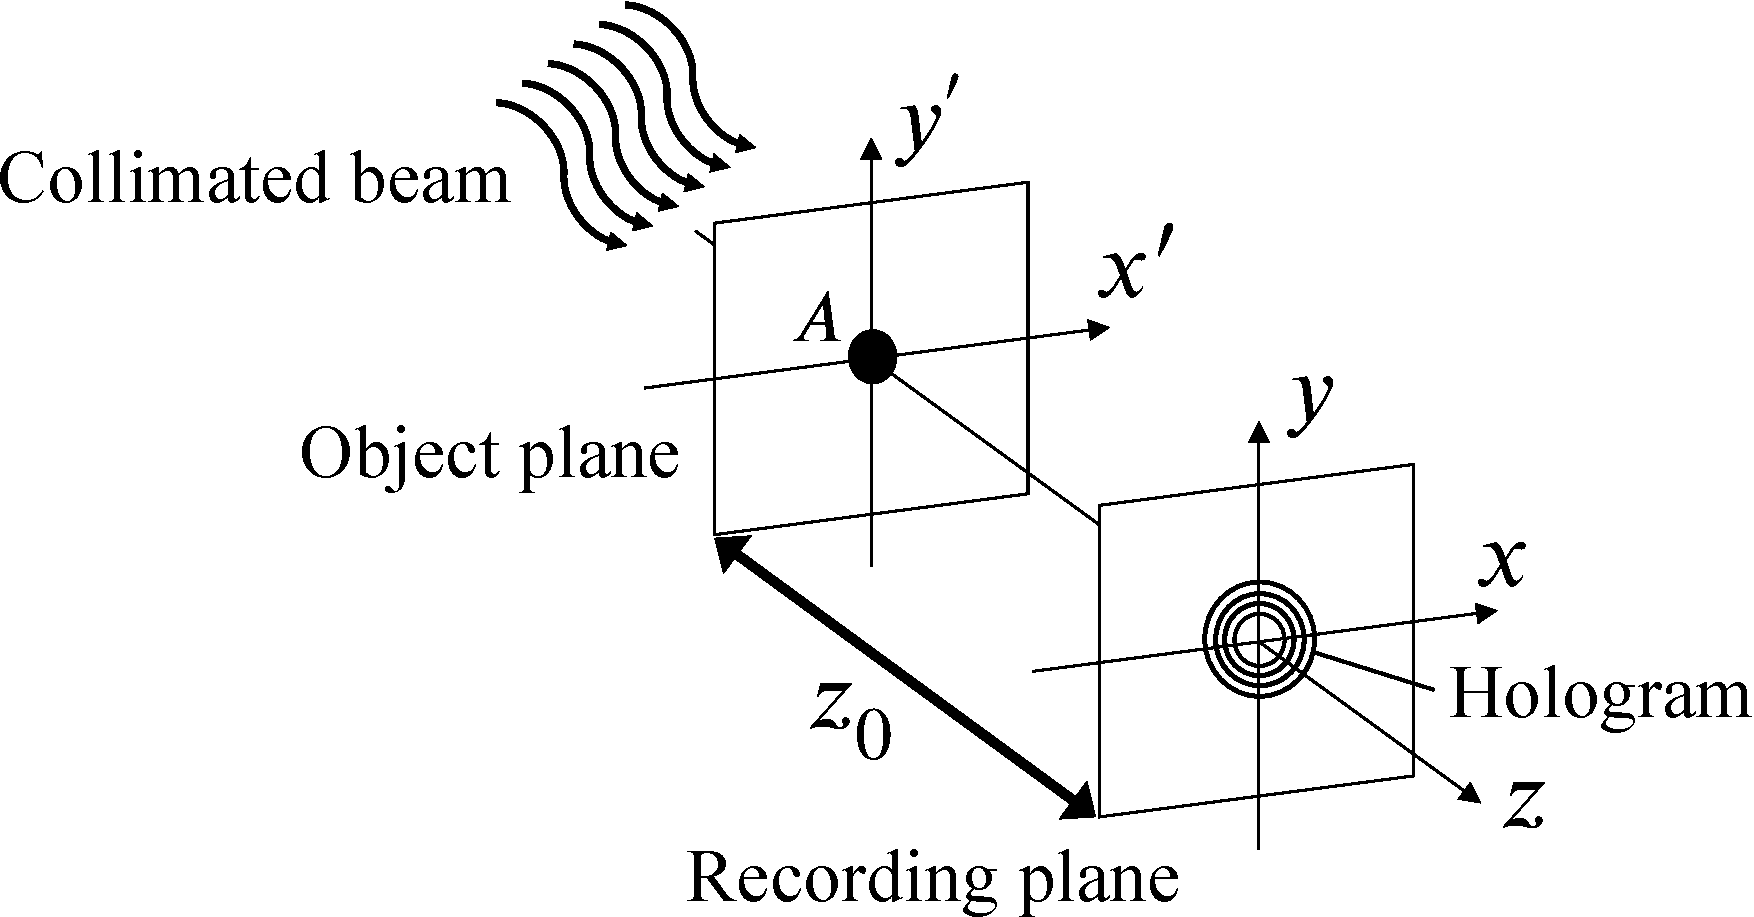
\includegraphics[width=0.8\linewidth]{./Figure/2_Theory/inline_holography.pdf}
    \caption{Schematic of in-line holography: collimated light illuminates a particle on the object plane, and appears as a diffraction pattern  on the recording plane. The irradiance of the complex amplitude on the recording plane is recorded as a hologram.}
    \label{fig:in-lineHolography}
\end{figure}

球形の3次元粒子は,ホログラムの記録時は3次元粒子中心に存在する物体面内の2次元円形として扱う.すなわち,$(x_p,y_p,z_p)$中心の半径 $a$の円は,以下の $z=z_p$上の形状関数$A(x,y;z_p)$として表現する.
\begin{equation}
    \label{th:particleShapeFunction}
    A(x,y;z_p) = \left\{
    \begin{aligned}
        &1 \quad \text{for } r_p \leq a \\
        &0 \quad \text{for } r_p > a
    \end{aligned}
    \right.
\end{equation}
ただし, $r_p=\sqrt{(x-x_p)^2+(y-y_p)^2}$である.今後この節では,便利のために$(x_p,y_p) = (0,0)$,$z_p = 0$とする.物体面$z=0$におけるコヒーレントな平行光の振幅を1,位相を0とすると,物体面における光複素振幅$\psi(x,y;0)$は,以下のようになる.
\begin{align}
    \psi(x,y;0) &= T(x,y)\cdot e^{\frac{2\pi \mathrm{j}}{\lambda}\cdot 0} \\
    &= 1 - A(x,y;0)
\end{align}
ここで,$T(x,y) = 1 - A(x,y;0)$は,物体面における透過関数と呼ばれる.これを$z_0$だけ伝搬して記録面の複素振幅$\psi(x,y;z_0)$を計算すると,式(\ref{th:fresneldiffraction}) に示すFresnel回折積分を用いて以下のようになる\cite{vikram}.
\begin{align}
    \label{th:particleComplexAmplitude}
    \psi(x,y;z_0) &= -\exp{\left( \frac{2\pi \mathrm{j}}{\lambda |z_0|} \right)} \left\{  
        1 + \frac{\mathrm{j}}{\lambda |z_0|} \exp{\left[ \frac{\pi \mathrm{j} \left( x^2+y^2 \right)}{\lambda |z_0|}\right] \tilde{A}\left( \frac{x}{\lambda |z_0|}, \frac{y}{\lambda |z_0|} \right) }
     \right\}
\end{align}
ただし, $\tilde{A}$は形状関数のフーリエ変換であり,以下の実数値関数で与えられる.
\begin{equation}
    \tilde{A}(\alpha,\beta) = \mathcal{F}\left\{ A \right\} = \pi a^2 \frac{2J_1(2\pi a \gamma)}{2\pi a \gamma}
\end{equation}
ここで, $\gamma = \sqrt{\alpha^2+\beta^2}$である.式(\ref{th:particleComplexAmplitude})では,以下の形式で用いられる.
\begin{equation}
    \label{th:fourierOfA}
    \tilde{A}\left( \frac{x}{\lambda |z_0|}, \frac{y}{\lambda |z_0|} \right)  =  \pi a^2 \frac{2J_1(2\pi a r/ \lambda |z_0|)}{2\pi a r/ \lambda |z_0|}
\end{equation}
ただし, $r=\sqrt{x^2+y^2}$である.結局,式(\ref{th:particleComplexAmplitude})は以下のようになる.
\begin{equation}
    \label{th:particleComplexAmplitude2}
    \psi(x,y;z_0) = -\exp{\left( \frac{2\pi \mathrm{j}}{\lambda |z_0|} \right)} \left\{  
        1 + \frac{\mathrm{j}}{\lambda |z_0|} \exp{\left[ \frac{\pi \mathrm{j} \left( x^2+y^2 \right)}{\lambda |z_0|}\right] \pi a^2 \frac{2J_1(2\pi a r/ \lambda |z_0|)}{2\pi a r/ \lambda |z_0|} }
     \right\}
\end{equation}

記録面のホログラム$I(x,y)$は,複素振幅の強度の2乗として以下のように計算できる.
\begin{equation}
    \label{th:irradiance}
    I(x,y) = |\psi(x,y;z_0)|^2 = \psi(x,y;z_0)\psi^*(x,y;z_0)
\end{equation}
これに式(\ref{th:particleComplexAmplitude})を代入して,以下を得る\cite{tyler1976}.
\begin{equation}
    \label{th:particleIrradiance}
    I(x,y) = 1 - \frac{2\pi a^2}{\lambda |z_0|} \sin{\left( \frac{\pi r^2}{\lambda |z_0|} \right)} \frac{2J_1(2\pi ar/\lambda |z_0|)}{2\pi ar / \lambda |z_0|} + \left( \frac{\pi a^2}{\lambda |z_0|} \right)^2 \left[ \frac{2J_1(2\pi ar/\lambda |z_0|)}{2\pi ar / \lambda |z_0|} \right]
\end{equation}

\subsubsection{粒子ホログラムの再生}\label{sec:holographicReconstruction}
\ref{sec:lightwaveProp}節で示した光伝搬計算を用いて,インラインホログラフィによる粒子像の再生を行う.ここで,ある平面波 $u(x,y;z)$ の光伝搬を $u*h_z$ のように表現する.光伝搬の演算 $*h_z$ は,その物理的性質から以下を満たす.
\begin{align}
    \label{th:lightPropOperation}
    \left( u * h_{z_1} \right) * h_{z_2} = u * h_{z_1 + z_2}
\end{align}
また,式(\ref{th:angularSpectrumTransferFunction}),式(\ref{th:fresnel-kirchhoff})より,以下を満たす.
\begin{equation}
    \label{th:lightPropOperation2}
    \overline{h_z} = h_{-z}
\end{equation}
形状関数 $A$ を持つ物体のホログラムは以下で表現される\cite{scott1987}.
\begin{align}
    \label{th:abstructParticleHologram}
    I(x,y) &= \left| \left( 1 - A(x,y) \right) * h_{z_0} \right|^2 \\
    &= \left|  1 - A(x,y)  * h_{z_0} \right|^2 \\
    \label{th:abstructParticleHologram2}
    &= 1 - \overline{A(x,y)}*\overline{h_{z_0}} - A(x,y)*h_{z_0} + \left| A(x,y) * h_{z_0} \right|^2
\end{align}
ここで,$1*h_{z_0}=1$ を用いたが,これは物体面における平行光の位相を $-2\pi z_0 /\lambda$ とすることで成立する.これはのちの計算を簡単にするための操作であり,このような位相のずれを導入してもホログラムおよびその再生像には影響しない.また,式(\ref{th:abstructParticleHologram2})の右辺第3項は十分小さいため省略する.ホログラムを $-z_0$ だけ逆伝搬して物体面の複素振幅を計算することで,物体の再生像を得る.
\begin{align}
    \label{th:particleReconstruction}
    \psi_{rec}(x,y;0) &= I(x,y) * h_{-z_0} \\
    &= 1 - \overline{A(x,y)}*\overline{h_{z_0}}*h_{z_0} - A(x,y)*h_{z_0}*h_{z_0} \\
    &= 1 - \overline{A(x,y)} - A(x,y)*h_{2z_0} \\
    \label{th:particleReconstruction2}
    &= \left( 1 - A(x,y) \right) + (1 - A(x,y))*h_{2z_0} - e^{\frac{2\pi \mathrm{j}z_0}{\lambda}}
\end{align}
ただし,$A(x,y)$が実数値関数であることを用いた.式(\ref{th:particleReconstruction2})の第1項は物体光を,第2項は双画像を,第3項は背景光を表す.双画像はホログラム記録時に位相分布が失われることで生じる.双画像はインラインホログラフィでは原理的に除去できないため,Off-axis法\cite{offaxis}や位相シフト法\cite{phaseshift},Gerchberg-Saxtonアルゴリズムを用いた位相回復法\cite{phaseretrieval}などが用いられる.

\subsection{2粒子ホログラムの局所特徴}
この節では,中心座標が $(x_{p1},y_{p1},z_{p1})$,半径 $a_1$ の粒子1と,中心座標が$(x_{p2},y_{p2},z_{p2})$,半径 $a_2$ の粒子2が近接したときに記録されるホログラフィックパターンの局所特徴について述べる.局所特徴とは画像上のある領域における幾何的な特徴を指す.すなわち,\ref{sec:holographicReconstruction}節で示したホログラムの3次元再生を行わず,ホログラムの画像としての特徴から直接粒子組の近接状態を識別することを目的とする.

はじめに,以下の条件を前提とする.
\begin{align}
    \sqrt{(x_{p1}-x_{p2})^2+(y_{p1}-y_{p2})^2} > a_1+a_2  \quad &\text{条件1: 点間の距離が半径の和より大きい} \\
    a_1 = a_2 \quad &\text{条件2: 二つの半径が等しい} \\
    z_{p1} = z_{p2} \quad &\text{条件3: 同じz座標上にある}
\end{align}
粒子1の形状関数を $A_1$,粒子2の形状関数を $A_2$ とする.形状関数 $A_i$ は,式(\ref{th:particleShapeFunction})にならって以下のように定義する.
\begin{equation}
    \label{th:eachParticleShapeFunction}
    A_i(x,y;z_{pi}) = \left\{
    \begin{aligned}
        &1 \quad \text{for } \sqrt{(x-x_{p2})^2+(y-y_{p2})^2} \leq a \\
        &0 \quad \text{for } \sqrt{(x-x_{p2})^2+(y-y_{p2})^2} > a
    \end{aligned}
    \right.
\end{equation}
これらの光伝搬による記録ホログラムを計算する.
\begin{align}
    \psi_{z_0} &= \mathcal{F}^{-1}\left\{ \mathcal{F}\{(1-A_1)(1-A_2)\}G(\alpha,\beta;z_{p1}) \right\} \\
    &= \mathcal{F}^{-1}\left\{ \mathcal{F}\{(1-A_1)+(1-A_2)-1\}G(\alpha,\beta;z_{p1}) \right\} \\
    & \begin{multlined} = \mathcal{F}^{-1}\left\{ \mathcal{F}\{1-A_1\}G(\alpha,\beta;z_{p1}) \right\} + \mathcal{F}^{-1}\left\{ \mathcal{F}\{1-A_2\}G(\alpha,\beta;z_{p1}) \right\} \\ - \mathcal{F}^{-1}\left\{ \mathcal{F}\{1\}G(\alpha,\beta;z_{p1}) \right\} \end{multlined}
\end{align}
ここで, $\mathcal{F}^{-1}\left\{ \mathcal{F}\{1-A_i\}G(\alpha,\beta;z_{p1}) \right\}$ は形状関数 $A_i$ を持つそれぞれの粒子が単独で光伝搬した際の複素振幅と等しい.また  $\mathcal{F}^{-1}\left\{ \mathcal{F}\{1\}G(\alpha,\beta;z_{p1}) \right\}$ は背景光の光伝搬を示す.それぞれは式(\ref{th:particleComplexAmplitude})より以下のように計算できる.
\begin{equation}
    \label{th:vikramEq4.8}
    \psi_{pi}(x,y) = -\exp{\left(\mathrm{j}\frac{2\pi}{\lambda}|z_{pi}|\right)} \left\{ 1 + \frac{\mathrm{j}}{\lambda |z_{pi}|} \exp{ \left[ \frac{\mathrm{j} \pi \left( x'^2 + y'^2 \right)}{\lambda |z_{pi}|} \right]} \tilde{A_1} \left(\frac{x'}{\lambda |z_{pi}|},\frac{y'}{\lambda |z_{pi}|} \right)  \right\}
\end{equation}
% vikram 4.8 式
ただし, $x' = x- x_{pi}$, $y' = y-y_{pi}$ である.また,背景光の光伝搬 $\mathcal{F}^{-1}\left\{ \mathcal{F}\{1\}G(\alpha,\beta;z_{p1}) \right\}$ は以下のようになる.
\begin{equation}
    \psi_b(x,y) = \mathcal{F}^{-1}\left\{ \mathcal{F}\{1\}G(\alpha,\beta;z_{p1}) \right\} = \exp{\left(\frac{2\pi \mathrm{j}z_{p1}}{\lambda}\right)}
\end{equation}

さて,今の条件を満たす任意の系は,一方の粒子の中心が $(x,y)$ 平面上の原点に存在するよう座標変換可能である.原点に固定した粒子を粒子1と呼び,他方の粒子を粒子2と呼ぶ.また,粒子2の中心座標は $(\Delta \xi, \Delta \eta)$ とする.すなわち,以下を満たす.
\begin{align}
    \left( x_{p1}, y_{p1} \right) &= (0,0) \\
    \left( x_{p2}, y_{p2} \right) &= (\Delta \xi ,\Delta \eta)
\end{align}
このように定めた粒子1の複素振幅を $\psi_{A_1}$,粒子2の複素振幅を $\psi_{A_1}$ とする.系をFig. \ref{fig:twoParticleHolography}に示す.

\begin{figure}[htbp]
    \centering
    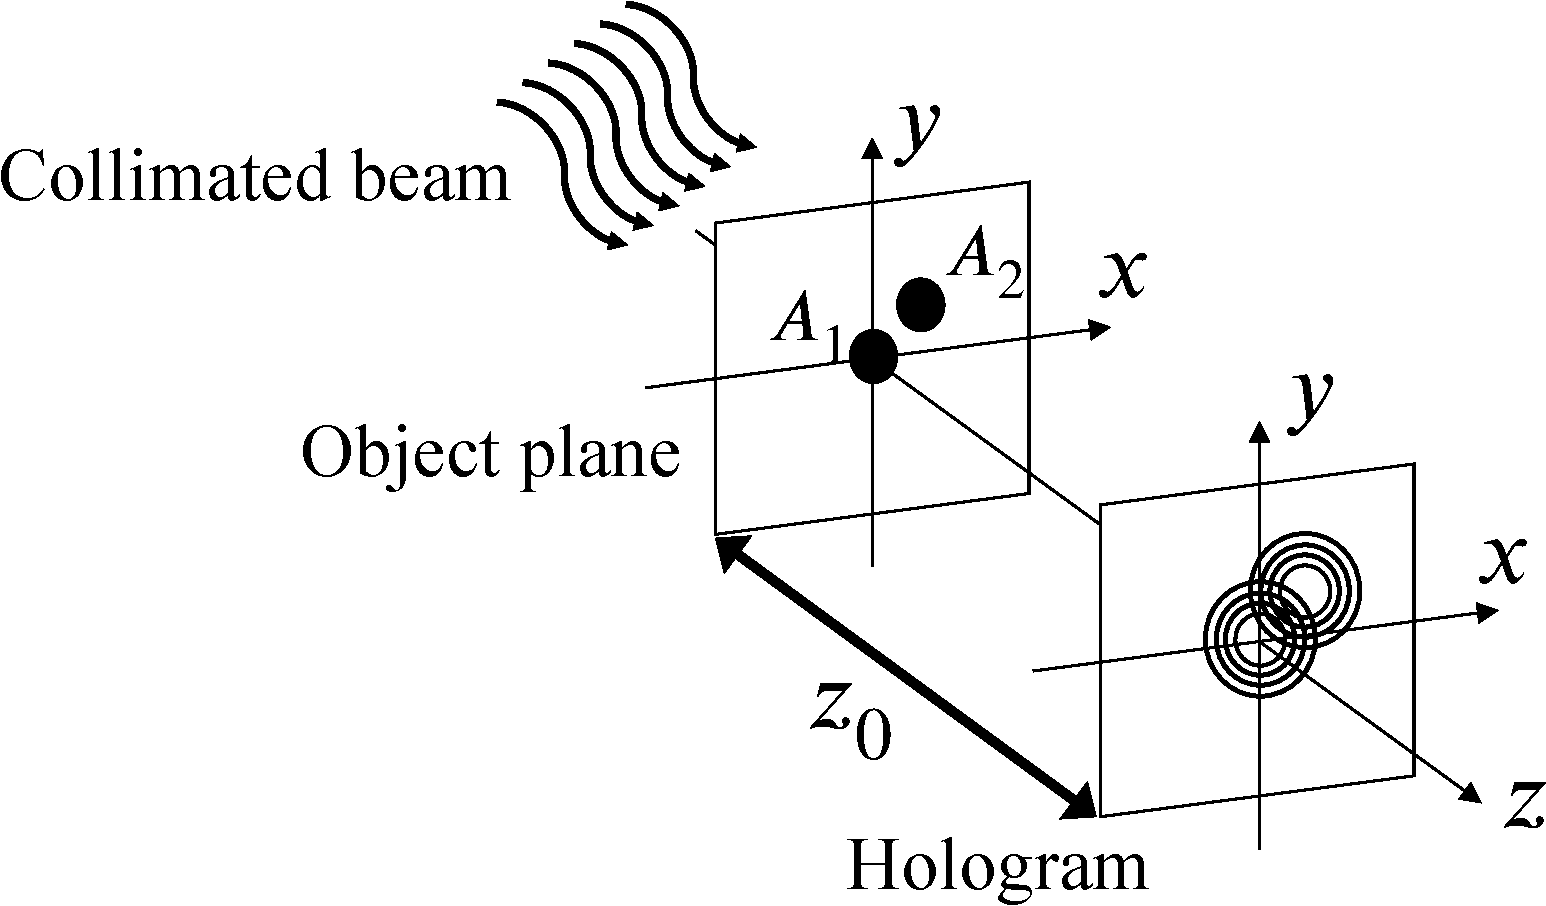
\includegraphics[width=0.8\linewidth]{./Figure/2_Theory/two_particle.pdf}
    \caption{Schematic of two-particle holography: two particles are located at $(0,0)$ and $(\Delta \xi, \Delta \eta)$, respectively. The depth position of the particles are the same, $z_{p1} = z_{p2}$.}
    \label{fig:twoParticleHolography}
\end{figure}

記録されるホログラム $I(x,y)$ は以下のように計算できる.
\begin{align}
    I(x,y) \coloneqq& \left|\psi_{A_1} + \psi_{A_2} - \psi_b \right|^2 \\
    \label{th:extraterms}
    =& |\psi_{A_1}|^2 + |\psi_{A_2}|^2 + 1 + 2\Re \left\{ \psi_{A_1} \overline{\psi_{A_2}} \right\} - 2\Re \left\{\overline{\psi_b}\left( \psi_{A_1} + \psi_{A_2} \right)\right\}
\end{align}
ここで,式(\ref{th:extraterms})右辺第3項以降を以下のように近似する.
\begin{equation}
    1 + 2\Re \left\{ \psi_{A_1} \overline{\psi_{A_2}} \right\} - 2\Re \left\{\overline{\psi_b}\left( \psi_{A_1} + \psi_{A_2} \right)\right\} = -1
\end{equation}
この近似の詳細については,付録\ref{sec:appendix_2particle}で述べる.結局,ホログラムは以下の式で与えられる.
\begin{equation}
    \label{th:2particleHologram}
    I(x,y) = |\psi_{A_1}|^2 + |\psi_{A_2}|^2 - 1
\end{equation}
したがって,同一物体面上同径近接粒子のホログラムは,二重露光ホログラフィで用いられていた以下の計算を適用可能になる\cite{doubleexposure}.

以降では,式(\ref{th:2particleHologram})に示したホログラムをフーリエ変換して得るスペクトル分布に現れる局所特徴について述べる.第一項および2項のフーリエ変換はそれぞれ以下で与えられる\cite{doubleexposure}.
\begin{align}
    \label{th:particle1Fourier}
    \varphi_{A_1}(\alpha,\beta)  = \mathcal{F}\left\{\left| \psi_{A_1} \right|\right\}  &\approx \cos{ \left( \pi \lambda z_0 \gamma^2 \right) }\tilde{A}(\alpha,\beta)  \\
    \label{th:particle2Fourier}
    \varphi_{A_2}(\alpha,\beta) = \mathcal{F}\left\{\left| \psi_{A_2} \right|\right\}   &\approx \cos{ \left( \pi \lambda z_0 \gamma^2 \right) }\tilde{A_2}(\alpha,\beta) \\
    &=\cos{ \left( \pi \lambda z_0 \gamma^2 \right) } \exp{\left( -2\pi \mathrm{j}\left( \alpha \Delta \xi + \beta \Delta \eta \right) \right)} \tilde{A}(\alpha,\beta)
\end{align}
ここで,$\tilde{A}$ は式(\ref{th:fourierOfA})を用いる.第二項のフーリエ変換 $\varphi_{A_2}$ の計算は,フーリエ変換のシフトルールによる.上の近似は,原点を除く点でのみ成立する.式(\ref{th:2particleHologram})第3項のフーリエ変換はデルタ関数であるため,これを省略して結局以下を得る.
\begin{align}
    \varphi(\alpha,\beta) &= \varphi_{A_1}(\alpha,\beta) + \varphi_{A_2}(\alpha,\beta) \\
    &= \tilde{A} \cos{\left( \pi \lambda z_0 \gamma^2 \right)} \cos{\left( \pi \left( \alpha \Delta \xi + \beta \Delta \eta \right) \right)} \exp{\left( \pi \mathrm{j} \left( \alpha \Delta \xi + \beta \Delta \eta \right) \right)}
\end{align}
したがって,スペクトル $S = |\varphi|^2$ は以下のようになる.
\begin{align}
    S(\alpha,\beta) &= \left| \varphi(\alpha,\beta) \right|^2 \\
    \label{th:2particleSpectrum}
    &= \left| \tilde{A} \right|^2 \cos^2{\left( \pi \lambda z_0 \gamma^2 \right)} \cos^2{\left( \pi \left( \alpha \Delta \xi + \beta \Delta \eta \right) \right)}
\end{align}









\subsection{位相回復ホログラフィ}


\subsection{畳み込みニューラルネットワークによる局所特徴識別}



